\subsubsection{Add an admin or a student assistant:}

\begin{figure}[H]
    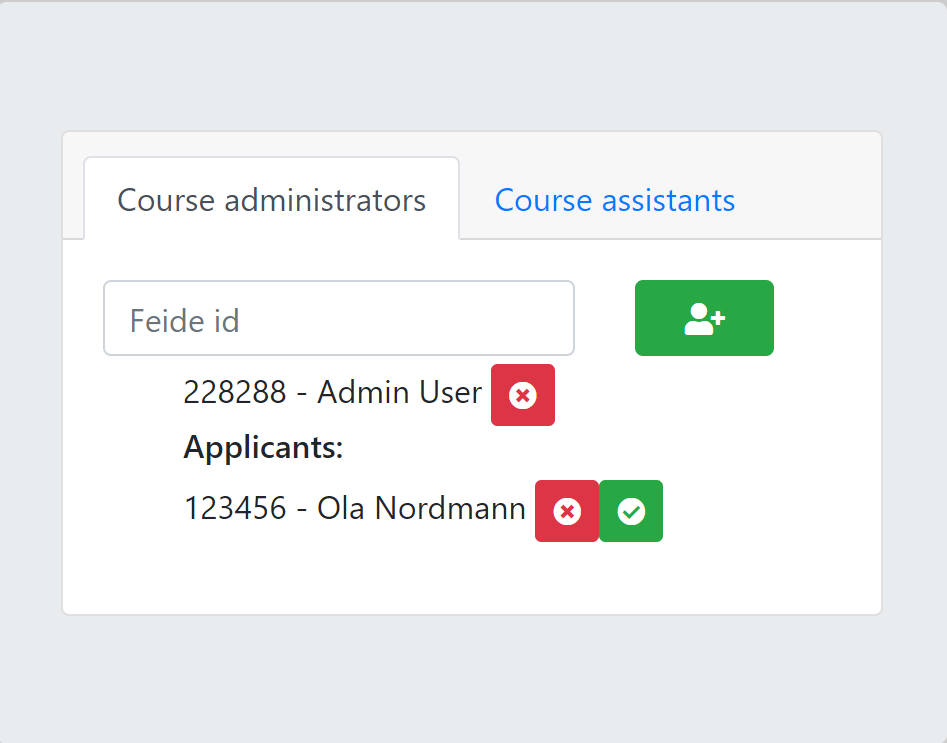
\includegraphics[width=0.70\linewidth]{userManual/adminImages/AdminRightsForCourse}
    \caption{}
    \label{fig:AdminRightsForCourse}
\end{figure}

\begin{userManualItemlist}
    \item[Step I.] Navigate to the admin dashboard page.
    \item[-] The following steps reference figure: \ref{fig:AdminRightsForCourse}
    \item[Step II.] Select "Course administrator" if you want to add an admin, or "Course assistants" if you want to add a student assistant.
    \item[Step III.] Type the user's Feide id inside the input field.
    \item[Step IV.] Click the green button.   
\end{userManualItemlist}

\subsubsection{To remove an admin or a student assistant:}
\begin{userManualItemlist}
    \item[Step I.] Navigate to the admin dashboard page.
    \item[-] The following steps reference figure: \ref{fig:AdminRightsForCourse} 
    \item[Step II.] Select "Course administrator" if you want to remove an admin, or "Course assistants" if you want to remove a student assistant.
    \item[Step III.] Click the red button next to the name of the person you want to remove.
\end{userManualItemlist}

\begin{figure}[H]
    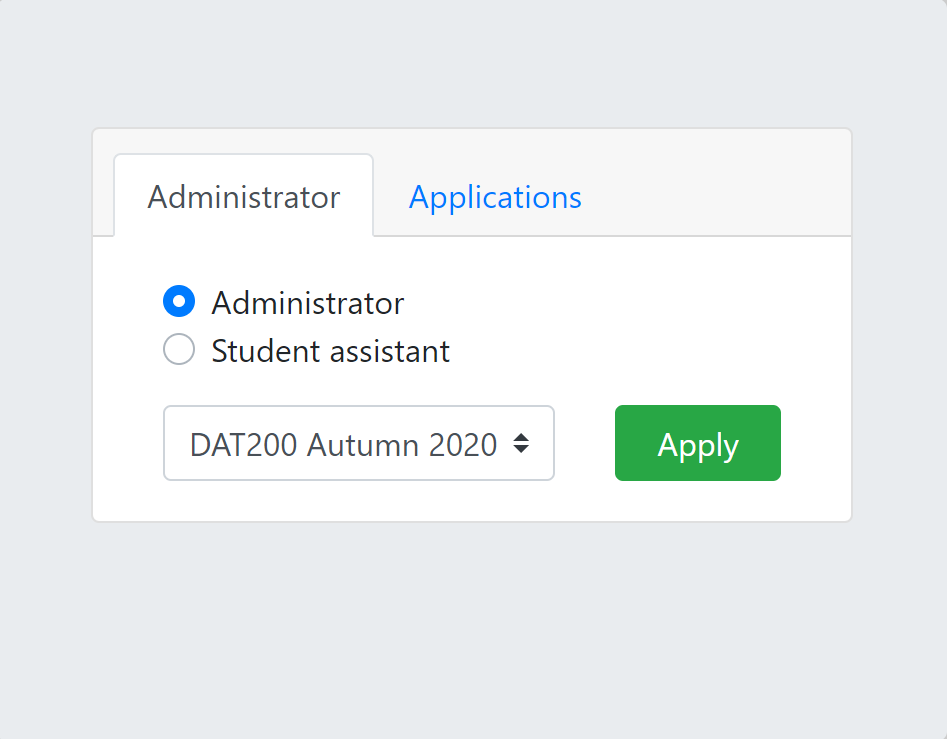
\includegraphics[width=0.70\linewidth]{userManual/adminImages/AdminApply}
    \caption{}
    \label{fig:AdminApply}
\end{figure}

\subsubsection{To request user rights for a course:}
\begin{userManualItemlist}
    \item[Step I.] Navigate to the admin dashboard page.
    \item[-] The following steps reference figure: \ref{fig:AdminApply} 
    \item[Step II.] Select "Administrator".
    \item[Step III.] Pick either "Administrator" or "Student assistant".
    \item[Step IV.] Select the course.
    \item[Step V.] Click the "Apply" button.   
\end{userManualItemlist}

